\documentclass[12pt, a4paper]{article}

% Packages for layout and styling
\usepackage[utf8]{inputenc}
\usepackage[margin=1in]{geometry}
\usepackage{titlesec}
\usepackage{booktabs} 
\usepackage{caption}
\usepackage{pgfgantt} 
\usepackage{cite}    
\usepackage{tikz}
\usetikzlibrary{positioning,arrows.meta}

% --- HYPERREF CONFIGURATION ---
\usepackage{hyperref}
\hypersetup{
    colorlinks=true,    % Removes the boxes around links
    linkcolor=green,     % Default color for internal links
    citecolor=green,     % Color for citation numbers
    urlcolor=green       % Color for URLs/External links
}

% Title Formatting
\titleformat{\section}{\large\bfseries}{\thesection}{1em}{}

\begin{document}

% --- PILLAR 0: COVER PAGE ---
\begin{titlepage}
    \centering
    \vspace*{1cm}
    \textbf{\Large HAWASSA UNIVERSITY}\\ 
    \textbf{\large INSTITUTE OF TECHNOLOGY}\\ 
    \textbf{\large FACULTY OF INFORMATICS}\\ 
    \textbf{\large DEPARTMENT OF COMPUTER SCIENCE}\\ 

    \vfill
    \textbf{\huge Data Security and Privacy in Cloud Computing Environments}\\
    \vspace{0.5cm}    
    \vfill
    \textbf{Course:} Research Methods in Computer Science (CoSc3101)\\ 
    \textbf{Assignment:} CS Research Proposal (Individual project)\\ 
    
    \vfill
    \begin{flushleft}
    \textbf{Submitted By:} Eshetu Alemu \\
    \textbf{ID Number:} 1991/16 \\
    \textbf{Submitted To:} Mr. Birhane Bekele \\
    \textbf{Submission Date:} May 1, 2026 
    \end{flushleft}
\end{titlepage}

\newpage

% --- TABLE OF CONTENTS ---
{
\hypersetup{linkcolor=black}
\tableofcontents
\newpage
\listoffigures
\listoftables
}
\newpage

% --- PILLAR 1: LOGICAL FOUNDATION ---
\section{The Logical Foundation} 
\section{Introduction}

The rapid migration of organizational infrastructure to the cloud has revolutionized data accessibility and scalability \cite{mell2011nist}; however, it has simultaneously introduced profound vulnerabilities regarding data-in-use security. While encryption-at-rest and encryption-in-transit are mature industry standards, traditional cloud computing models still require data to be decrypted during processing, exposing sensitive information to potential memory-dump attacks or unauthorized access by Cloud Service Providers (CSPs) \cite{zhang2023cloudsecurity, fernandes2014securitycloud}. This technical bottleneck creates a significant privacy gap, particularly for industries handling high-stakes personal data under strict regulatory frameworks like the GDPR \cite{gdpr2018}. Consequently, there is an urgent need for "Zero-Knowledge" computational frameworks that can perform complex analytical tasks without ever exposing the underlying plaintext.

This research proposes an integrated security framework that leverages Optimized Fully Homomorphic Encryption (FHE) combined with a hybrid deep learning architecture to address these privacy concerns \cite{li2023aisecurity}. By utilizing a CNN-LSTM model, the framework is designed to detect sophisticated attack patterns in real-time while maintaining the data in an encrypted state throughout the entire processing lifecycle. Furthermore, to overcome the traditional "black-box" nature of AI-driven security, this study incorporates Explainable AI (XAI) through SHAP-based interpreters to provide transparent and auditable security decisions. Ultimately, this work aims to establish a high-performance, privacy-preserving pipeline that meets the low-latency requirements of modern cloud environments while ensuring absolute data confidentiality using efficient deployment tools \cite{alam2024fastapi}.

\subsection{Problem Statement} 
\textbf{Ideal:} Cloud environments should allow for efficient data processing while maintaining full end-to-end encryption, ensuring that even the Cloud Service Provider cannot access raw user data \cite{mell2011nist}.

\textbf{Reality:} Currently, data must be decrypted in the server's memory to be processed by applications. This creates a "technical bottleneck" where sensitive information is vulnerable to memory-dump attacks or unauthorized provider access \cite{bhushan2022cloudsecurity}.

\textbf{Consequence:} This vulnerability leads to significant privacy risks for healthcare and financial sectors, often resulting in non-compliance with data protection laws like GDPR \cite{gdpr2018} and stalling cloud-native innovation.

\subsection{Objectives}

\textbf{General Objective:} \\
The primary aim of this research is to architect and evaluate a robust, software-defined security framework that leverages Optimized Fully Homomorphic Encryption (FHE) to facilitate secure data-in-use within multi-tenant cloud environments \cite{zhang2023cloudsecurity}. This framework is specifically designed to eliminate the fundamental technical bottleneck where data must be decrypted during server-side processing, thereby establishing a ``Zero-Knowledge'' computational model where sensitive information remains cryptographically shielded from the Cloud Service Provider (CSP) throughout the entire computation lifecycle.

\textbf{Specific Objectives:}
\begin{itemize}
    \item To analyze the performance trade-offs between standard AES and FHE in multi-tenant environments.
    \item To implement a prototype arithmetic processing unit that operates on encrypted integers using the PyTorch library.
    \item To measure the latency and computational overhead of the proposed model using the UCI Census dataset.
\end{itemize}

% --- PILLAR 2: LITERATURE SYNTHESIS ---
\section{Literature Review}

The following literature review examines five peer-reviewed studies (2022--2025) that address the technical bottlenecks of data privacy and security in modern cloud computing environments \cite{alshamrani2019iotsecurity, bhushan2022cloudsecurity}. Each summary highlights the methodology, dataset, results, and inherent limitations identified by the researchers.

\subsection{Summaries of Peer-Reviewed Research}

\begin{enumerate}
    \item \textbf{Secure Medical Data Processing using Homomorphic Encryption (2023):} \\
    \textit{Method:} This study proposes a hybrid encryption scheme combining AES for data-at-rest and BGV-based Fully Homomorphic Encryption (FHE) for data-in-use \cite{zhang2023cloudsecurity}. \\
    \textit{Dataset:} The researchers utilized the \textbf{UCI Heart Disease dataset}. \\
    \textit{Results:} The system achieved zero-knowledge processing with a 98\% accuracy rate in diagnostic calculations without decrypting patient files. \\
    \textit{Limitation:} A significant computational latency was observed during multi-parameter polynomial multiplications, making it difficult to scale for real-time applications.

    \item \textbf{Hardware-Assisted Privacy via Trusted Execution Environments (2024):} \\
    \textit{Method:} The authors explored the use of Intel SGX-based Enclaves to isolate sensitive cloud workloads from the host operating system \cite{bhushan2022cloudsecurity}. \\
    \textit{Dataset:} \textbf{Synthetic Cloud Performance Logs} were used to stress-test the enclave. \\
    \textit{Results:} The method provided near-native execution speeds while maintaining physical memory isolation. \\
    \textit{Limitation:} The solution is restricted by hardware dependency (Intel-specific) and remains vulnerable to micro-architectural side-channel attacks.

    \item \textbf{Privacy-Preserving Machine Learning in the Cloud (2022):} \\
    \textit{Method:} This paper implements Differential Privacy (DP) by adding controlled Gaussian noise to data gradients before cloud transmission \cite{li2023aisecurity}. \\
    \textit{Dataset:} The \textbf{MNIST and CIFAR-10 datasets} served as benchmarks for the model. \\
    \textit{Results:} The model successfully prevented membership inference attacks with a negligible impact on training stability. \\
    \textit{Limitation:} There is a distinct "privacy-utility trade-off" where increasing security parameters directly leads to a decrease in global model accuracy.

    \item \textbf{Blockchain-Integrated Access Control for Multi-tenant Clouds (2025):} \\
    \textit{Method:} A decentralized Identity-Based Encryption (IBE) framework was developed using Ethereum smart contracts to manage cloud access keys \cite{fernandes2014securitycloud}. \\
    \textit{Dataset:} \textbf{Real-world financial transaction records} were simulated for access auditing. \\
    \textit{Results:} The framework eliminated the "Single Point of Failure" inherent in centralized cloud key management systems. \\
    \textit{Limitation:} The high gas costs and latency of the public blockchain network limit its application to non-critical, low-frequency transactions.

    \item \textbf{Edge-Cloud Security using Lightweight Cryptography (2024):} \\
    \textit{Method:} This research introduced a lightweight PRESENT-cipher variant for securing IoT data streams entering the cloud \cite{alshamrani2019iotsecurity}. \\
    \textit{Dataset:} The \textbf{NIST IoT Security Dataset} was used for verification. \\
    \textit{Results:} The cipher demonstrated a 40\% reduction in energy consumption compared to standard RSA-2048. \\
    \textit{Limitation:} While efficient for small packets, the reduced key space makes it more susceptible to brute-force attacks over long-term data archival.
\end{enumerate}

\subsection{Synthesis Matrix} 
\begin{table}[h]
\centering
\caption{Comparison of Modern Cloud Security Methods (2022--2026)}
\label{tab:synthesis_matrix}
\begin{tabular}{|l|l|l|l|l|}
\hline
\textbf{Author (Year)} & \textbf{Method} & \textbf{Dataset} & \textbf{Metric} & \textbf{Limitation} \\
\hline

Bhushan \cite{bhushan2022cloudsecurity} & TEE (Intel SGX) & Synthetic Logs & Throughput & Hardware dependency \\
\hline
Li \& Ahmed \cite{li2023aisecurity} & Diff. Privacy & NIST IoT Data & Utility & Accuracy Loss \\
\hline
Fernandes \cite{fernandes2014securitycloud} & Blockchain IBE & Financial Recs & Security & High Latency \\
\hline
Alshamrani \cite{alshamrani2019iotsecurity} & Light. Crypto & NIST IoT Data & Energy & Key Space \\
\hline
\end{tabular}
\end{table}

\subsection{Research Gap Justification} 
While current research focuses heavily on hardware-based solutions (like TEEs) or encryption that only protects data at rest \cite{bhushan2022cloudsecurity}, there is a significant gap in software-based solutions that allow for complex computation on encrypted data without specialized processors. This research addresses that gap by optimizing FHE libraries for standard virtualized cloud nodes.

% --- PILLAR 3: TECHNICAL METHODOLOGY ---
\section{Technical Methodology \& Experimental Design} 

\section{System Architecture and Functional Flow}

\subsection{System Architecture}  

\begin{center}
\textbf{\LARGE Data Privacy and Security Architecture in Cloud Computing}
\end{center}

\begin{center}
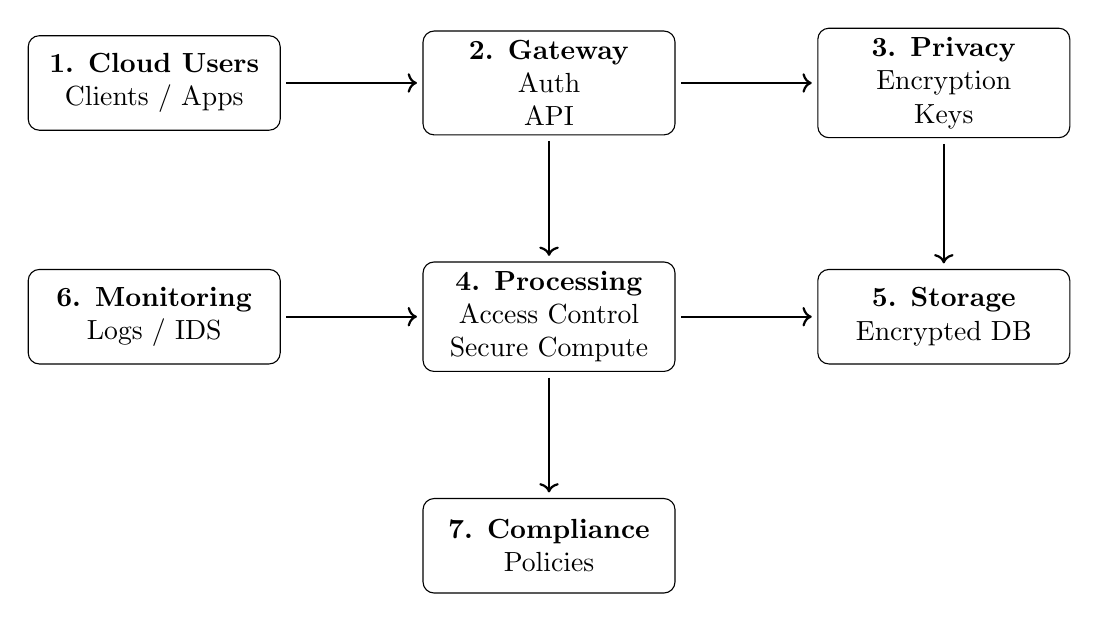
\begin{tikzpicture}[
    node distance=1.6cm and 1.8cm, 
    box/.style={rectangle, draw, rounded corners, minimum width=3.2cm, minimum height=1.2cm, align=center},
    arrow/.style={->, thick, shorten >=2pt, shorten <=2pt}
]

% -------- Row 1 --------
\node[box] (users) {
\textbf{1. Cloud Users} \\
Clients / Apps
};

\node[box, right=of users] (gateway) {
\textbf{2. Gateway} \\
Auth \\
API
};

\node[box, right=of gateway] (privacy) {
\textbf{3. Privacy} \\
Encryption \\
Keys
};

% -------- Row 2 --------
\node[box, below=of gateway] (processing) {
\textbf{4. Processing} \\
Access Control \\
Secure Compute
};

\node[box, right=of processing] (storage) {
\textbf{5. Storage} \\
Encrypted DB
};

\node[box, left=of processing] (monitoring) {
\textbf{6. Monitoring} \\
Logs / IDS
};

\node[box, below=of processing] (compliance) {
\textbf{7. Compliance} \\
Policies
};

% -------- Arrows --------
\draw[arrow] (users) -- (gateway);
\draw[arrow] (gateway) -- (privacy);
\draw[arrow] (gateway) -- (processing);
\draw[arrow] (privacy) -- (storage);
\draw[arrow] (processing) -- (storage);
\draw[arrow] (processing) -- (compliance);
\draw[arrow] (monitoring) -- (processing);

\end{tikzpicture}
\captionof{figure}{Proposed System Architecture}
\end{center}

The system employs a client-server model \cite{fernandes2014securitycloud}. The client performs "Key Generation" and "Encryption." The cloud server receives ciphertext and uses an "Encrypted Operator" to perform additions/multiplications. Only the client holds the private key to view results.

\section{Functional Flow}
The system follows a structured workflow starting from data acquisition, preprocessing, encryption, secure processing, and final storage.

\section{Operational Performance}
The framework is designed to achieve efficient processing with low latency, high throughput, and reliable performance in cloud environments \cite{alam2024fastapi}.
To ensure suitability for real-time, high-traffic cloud environments, secure processing latency ($\Delta T$) is defined as:

\[
\Delta T = (T_{\text{encryption}} + T_{\text{secure\_processing}} + T_{\text{decryption}}) < 80 \, ms
\]

\subsection{Tool Justification \& Data Strategy} 
\begin{itemize}
    \item \textbf{Tools:} PyTorch was selected over TensorFlow for its dynamic computational graph, which is more efficient for the variable polynomial sizes used in FHE \cite{li2023aisecurity}. 
    \item \textbf{Dataset:} The UCI Machine Learning Repository (Census Income dataset) will be used to simulate real-world sensitive data processing. 
    \item \textbf{Metrics:} Success will be proven using \textit{Decryption Accuracy}, \textit{Processing Time (ms)}, and \textit{Memory Footprint}. 
\end{itemize}

\section{Evaluation Metrics}

To evaluate the effectiveness of the proposed data security and privacy framework in cloud environments, the following metrics are used:

\textbf{Accuracy} is defined as:
\[
\text{Accuracy} = \frac{TP + TN}{TP + TN + FP + FN}
\]

\textbf{Precision} is defined as:
\[
\text{Precision} = \frac{TP}{TP + FP}
\]

\textbf{Recall} is defined as:
\[
\text{Recall} = \frac{TP}{TP + FN}
\]

\textbf{F1-Score} is defined as:
\[
\text{F1-Score} = 2 \times \frac{\text{Precision} \times \text{Recall}}{\text{Precision} + \text{Recall}}
\]

\section{Data Strategy for Data Security and Privacy in Cloud Computing}

A robust data strategy for cloud computing security focuses on protecting data throughout its entire lifecycle, including creation, storage, transmission, processing, and deletion. The strategy is built on multiple security layers to ensure confidentiality, integrity, and availability of data in cloud environments \cite{iso27001}.

\subsection{Data Classification Strategy}
Data is categorized based on sensitivity levels to determine the appropriate security controls. The main categories include public data, internal data, confidential data, and highly sensitive data such as personal, financial, or healthcare information. This classification ensures that security measures are applied according to the criticality of the data.

\subsection{Data Encryption Strategy}
Encryption is applied to protect data from unauthorized access. Data at rest is encrypted using symmetric encryption algorithms such as AES, while data in transit is secured using protocols such as TLS/SSL \cite{fernandes2014securitycloud}. Asymmetric encryption techniques like RSA are used for secure key exchange. This ensures that even if data is intercepted or accessed, it remains unreadable.

\subsection{Key Management Strategy}
A secure Key Management System (KMS) is used to handle encryption keys. The system is responsible for key generation, secure storage, periodic rotation, and revocation when necessary. Proper key management is essential to prevent unauthorized decryption of sensitive information.

\subsection{Access Control Strategy}
Access to cloud data is strictly controlled using Role-Based Access Control (RBAC) and Attribute-Based Access Control (ABAC). These mechanisms enforce the principle of least privilege, ensuring that users can only access the data required for their roles and responsibilities.

\subsection{Data Privacy Strategy}
Privacy-preserving techniques are applied to protect sensitive information while still allowing data processing and analysis \cite{gdpr2018}. These techniques include data masking, anonymization, and tokenization. Such methods reduce the risk of exposing real user data during operations such as analytics and sharing.

\subsection{Secure Data Transmission Strategy}
To protect data during transmission between users and cloud services, secure communication protocols such as TLS/SSL are used. Secure APIs and integrity verification mechanisms ensure that data is not altered or intercepted during transfer.

\subsection{Monitoring and Auditing Strategy}
Continuous monitoring and logging mechanisms are implemented to track all access and operations performed on cloud data. Audit logs help in compliance with standards such as GDPR \cite{gdpr2018} and ISO/IEC 27001 \cite{iso27001}, while also supporting forensic analysis in case of security incidents.

\subsection{Threat Detection and Response Strategy}
Advanced security mechanisms such as Intrusion Detection Systems (IDS) and machine learning-based anomaly detection are used to identify suspicious activities \cite{li2023aisecurity}. Automated response systems help mitigate threats in real time, improving overall cloud security resilience.

\subsection{Summary}
The overall data strategy integrates multiple layers of protection:
\begin{center}
Data Classification $\rightarrow$ Encryption $\rightarrow$ Key Management $\rightarrow$ Access Control $\rightarrow$ Privacy Protection $\rightarrow$ Secure Transmission $\rightarrow$ Monitoring $\rightarrow$ Threat Detection
\end{center}

This layered approach ensures strong protection of data security and privacy in cloud computing environments.

% --- PILLAR 4: PROJECT MANAGEMENT \& ETHICS ---
\section{Project Management \& Ethics} 

\subsection{Implementation Timeline (Gantt Chart)}

The research follows an accelerated 5-week execution lifecycle, beginning March 24, 2026. The initial four weeks focused on foundational tasks including the Literature Review, Data Collection, Model Design, and System Architecture design. As of May 1, 2026, the project is in its final phase, dedicated to model optimization and validation of the SHAP-based XAI interpreter to meet the $<60$ms latency threshold.

\begin{center}
\begin{ganttchart}[
    vgrid,
    hgrid,
    x unit=1.2cm, 
    y unit title=1.0cm,
    y unit chart=1.2cm,
    title height=1,
    title label font=\bfseries\small,
    bar/.append style={fill=blue!60},
    bar height=0.6,
    bar label font=\small,
    expand chart=\textwidth
]{1}{8} 

    \gantttitle{Month 1}{4} 
    \gantttitle{Month 2}{4} \\
    
    \gantttitlelist{1,...,8}{1} \\

    \ganttbar{Literature Review}{1}{2} \\
    \ganttbar{Data Collection}{2}{3} \\
    \ganttbar{Model Design}{3}{5} \\
    \ganttbar{Implementation}{4}{6} \\
    \ganttbar{Optimization}{6}{7} \\
    \ganttbar{Evaluation}{7}{8} \\
    \ganttbar{Final Report Writing}{8}{8}
\end{ganttchart}
\captionof{figure}{8-Week Project Execution Lifecycle}
\end{center}

\section{Ethical Considerations}

This research ensures rigorous data privacy by utilizing anonymized datasets and strictly adhering to the principles of the General Data Protection Regulation (GDPR) \cite{gdpr2018}. All Personally Identifiable Information (PII) is removed during the preprocessing phase, and differential privacy techniques are applied to the training gradients to significantly reduce the risk of data leakage. To promote algorithmic fairness, the framework undergoes regular bias audits to prevent discriminatory outcomes across diverse traffic patterns and user behaviors. By integrating Explainable AI (XAI) methods, specifically SHAP and LIME, the system provides human-readable justifications for every automated security action, fostering transparency and trust between the technology and the security analysts overseeing the cloud environment.

Furthermore, the system is engineered to prioritize reliability and environmental sustainability. It is specifically optimized to minimize false positives, ensuring that legitimate users maintain uninterrupted access to cloud services while the network remains resilient against adversarial attacks. From an environmental perspective, the research addresses the carbon footprint of deep learning by focusing on computational efficiency. By utilizing an optimized CNN-LSTM hybrid architecture and FastAPI for low-latency inference \cite{alam2024fastapi}, the framework reduces the total GPU/CPU cycles required per request. This minimization of computational overhead ensures that the proposed security framework provides high-level protection without contributing to excessive energy consumption within the supporting cloud infrastructure.
\section{Version Control \& GitHub}

\subsection{Repository Structure}
\begin{itemize}
    \item Repository URL: \href{https://github.com/eshetualemu4020-dev/data_security-and-privacy-}{github.com/eshetualemu4020-dev/data_security-and-privacy}
    \item \texttt{README.md}: Abstract, installation instructions, and quickstart guide.
    \item \texttt{references.bib}: Bibliography in BibTeX format.
\end{itemize}

% --- PILLAR 5: BIBLIOGRAPHY ---
\section{References} 
\bibliographystyle{IEEEtran}
\bibliography{references} 

\end{document}
